\documentclass[aspectratio=169]{beamer}

\usetheme{Boadilla}
\setbeamertemplate{navigation symbols}{}

\usepackage[T1]{fontenc}
\usepackage[utf8]{inputenc}
\usepackage{booktabs}
\usepackage{array}
\usepackage{amsmath}
\usepackage{graphicx}
\usepackage{xcolor}

% ── Custom color palette: navy blue + slate ──────────────────────────────────
\definecolor{qNavy}{RGB}{15, 40, 90}       % deep navy
\definecolor{qMid}{RGB}{0, 100, 180}       % medium blue (accent)
\definecolor{qLight}{RGB}{220, 232, 245}   % very light blue (block bg)
\definecolor{qGold}{RGB}{200, 160, 40}     % warm accent for highlights

% Frame title bar
\setbeamercolor{frametitle}{bg=qNavy, fg=white}
\setbeamercolor{frametitle right}{bg=qNavy}

% Title page
\setbeamercolor{title}{fg=white}
\setbeamercolor{subtitle}{fg=qLight}
\setbeamercolor{author}{fg=qLight}
\setbeamercolor{date}{fg=qLight}
\setbeamercolor{titlegraphic}{fg=white}

% Footer / header palette
\setbeamercolor{palette primary}{bg=qNavy, fg=white}
\setbeamercolor{palette secondary}{bg=qMid, fg=white}
\setbeamercolor{palette tertiary}{bg=qNavy!70, fg=white}
\setbeamercolor{palette quaternary}{bg=qNavy, fg=white}

% Bullets
\setbeamercolor{itemize item}{fg=qMid}
\setbeamercolor{itemize subitem}{fg=qMid!70}
\setbeamercolor{enumerate item}{fg=qMid}

% Block
\setbeamercolor{block title}{bg=qNavy, fg=white}
\setbeamercolor{block body}{bg=qLight, fg=black}

% Structure (section, etc.)
\setbeamercolor{structure}{fg=qMid}

% Title page background
\setbeamercolor{background canvas}{bg=white}

% Make title slide have navy background
\setbeamertemplate{title page}{%
  \begin{tikzpicture}[remember picture, overlay]
    \fill[qNavy] (current page.north west) rectangle (current page.south east);
  \end{tikzpicture}%
  \vspace{2em}
  \begin{center}
    {\Large\color{white}\textbf{\inserttitle}}\\[0.5em]
    {\small\color{qLight}\insertsubtitle}\\[1.5em]
    {\color{qLight}\insertauthor}\\[0.3em]
    {\color{qLight}\insertdate}
  \end{center}
}

\usepackage{tikz}

\title{Strategy-Space Modeling for Interpretable Quant Research}
\subtitle{From Linear Combination to ML-Guided Allocation on GLD}
\author{Joon Chun}
\date{April 2026}

\begin{document}

% ── Slide 1: Title ──────────────────────────────────────────────────────────
\begin{frame}
  \titlepage
\end{frame}

% ── Slide 2: Starting Point ──────────────────────────────────────────────────
\begin{frame}{Starting Point}
  \begin{itemize}
    \item The project started from a mathematical question, not a trading rule.
    \item In class, we studied model selection using polynomial basis functions:
    \[
      1,\ x,\ x^2,\ \dots,\ x^d
    \]
    \item That raised the main idea:
    \[
      \text{Can trading strategies also be treated as basis functions?}
    \]
    \item If a strategy maps a market state into a numerical score,
          it can be evaluated across dates and placed into a design matrix.
  \end{itemize}
\end{frame}

% ── Slide 3: Function Space Analogy ─────────────────────────────────────────
\begin{frame}{Function Space Analogy}
  \small
  \begin{tabular}{lll}
    \toprule
    Concept & Polynomial Model & Strategy Model \\
    \midrule
    basis function  & \(1, x, x^2, \dots\)   & strategy signal functions \\
    data point      & \(x_i\)                 & market state at date \(t_i\) \\
    matrix entry    & \(\phi_j(x_i)\)         & strategy score \(s_j(t_i)\) \\
    model selection & choose degree / penalty & choose strategy / penalty \\
    target          & observed \(y_i\)        & future cumulative return \\
    \bottomrule
  \end{tabular}

  \vspace{0.8em}
  Core design matrix:
  \[
    A_{ij} = \phi_j(\text{market state at } t_i)
  \]

  \vspace{0.4em}
  Each column is a strategy function evaluated over time.
  Each row is one trading day.
\end{frame}

% ── Slide 4: Four Strategy Families ─────────────────────────────────────────
\begin{frame}{Four Trading Strategy Families}
  These are strategies practitioners actually use on price data.

  \vspace{0.6em}
  \begin{tabular}{lll}
    \toprule
    Strategy & Signal Type & Core Idea \\
    \midrule
    Adaptive Band            & continuous & price position inside rolling bands \\
    MA Crossover             & continuous & short vs.\ long moving average gap \\
    Adaptive Volatility Band & continuous & volatility regime from H-L-C range \\
    Fear-Greed Candle-Volume & event      & large candle + volume spike \\
    \bottomrule
  \end{tabular}

  \vspace{0.8em}
  Each strategy maps a market state to a number (score).\\
  That number becomes one column of matrix \(A\).
\end{frame}

% ── Slide 5: Strategy 1 ──────────────────────────────────────────────────────
\begin{frame}{Strategy 1: Adaptive Band}
  \begin{columns}[T]
    \begin{column}{0.40\textwidth}
      \small
      \textbf{Signal type: continuous}
      \vspace{0.5em}
      \begin{itemize}
        \item Price normalized relative to a rolling moving average
        \item Upper and lower bands placed at scaled thresholds
        \item Score: how far price sits from the band midpoint
        \item Buy zone: price near or below lower band
        \item Sell zone: price near or above upper band
      \end{itemize}
    \end{column}
    \begin{column}{0.57\textwidth}
      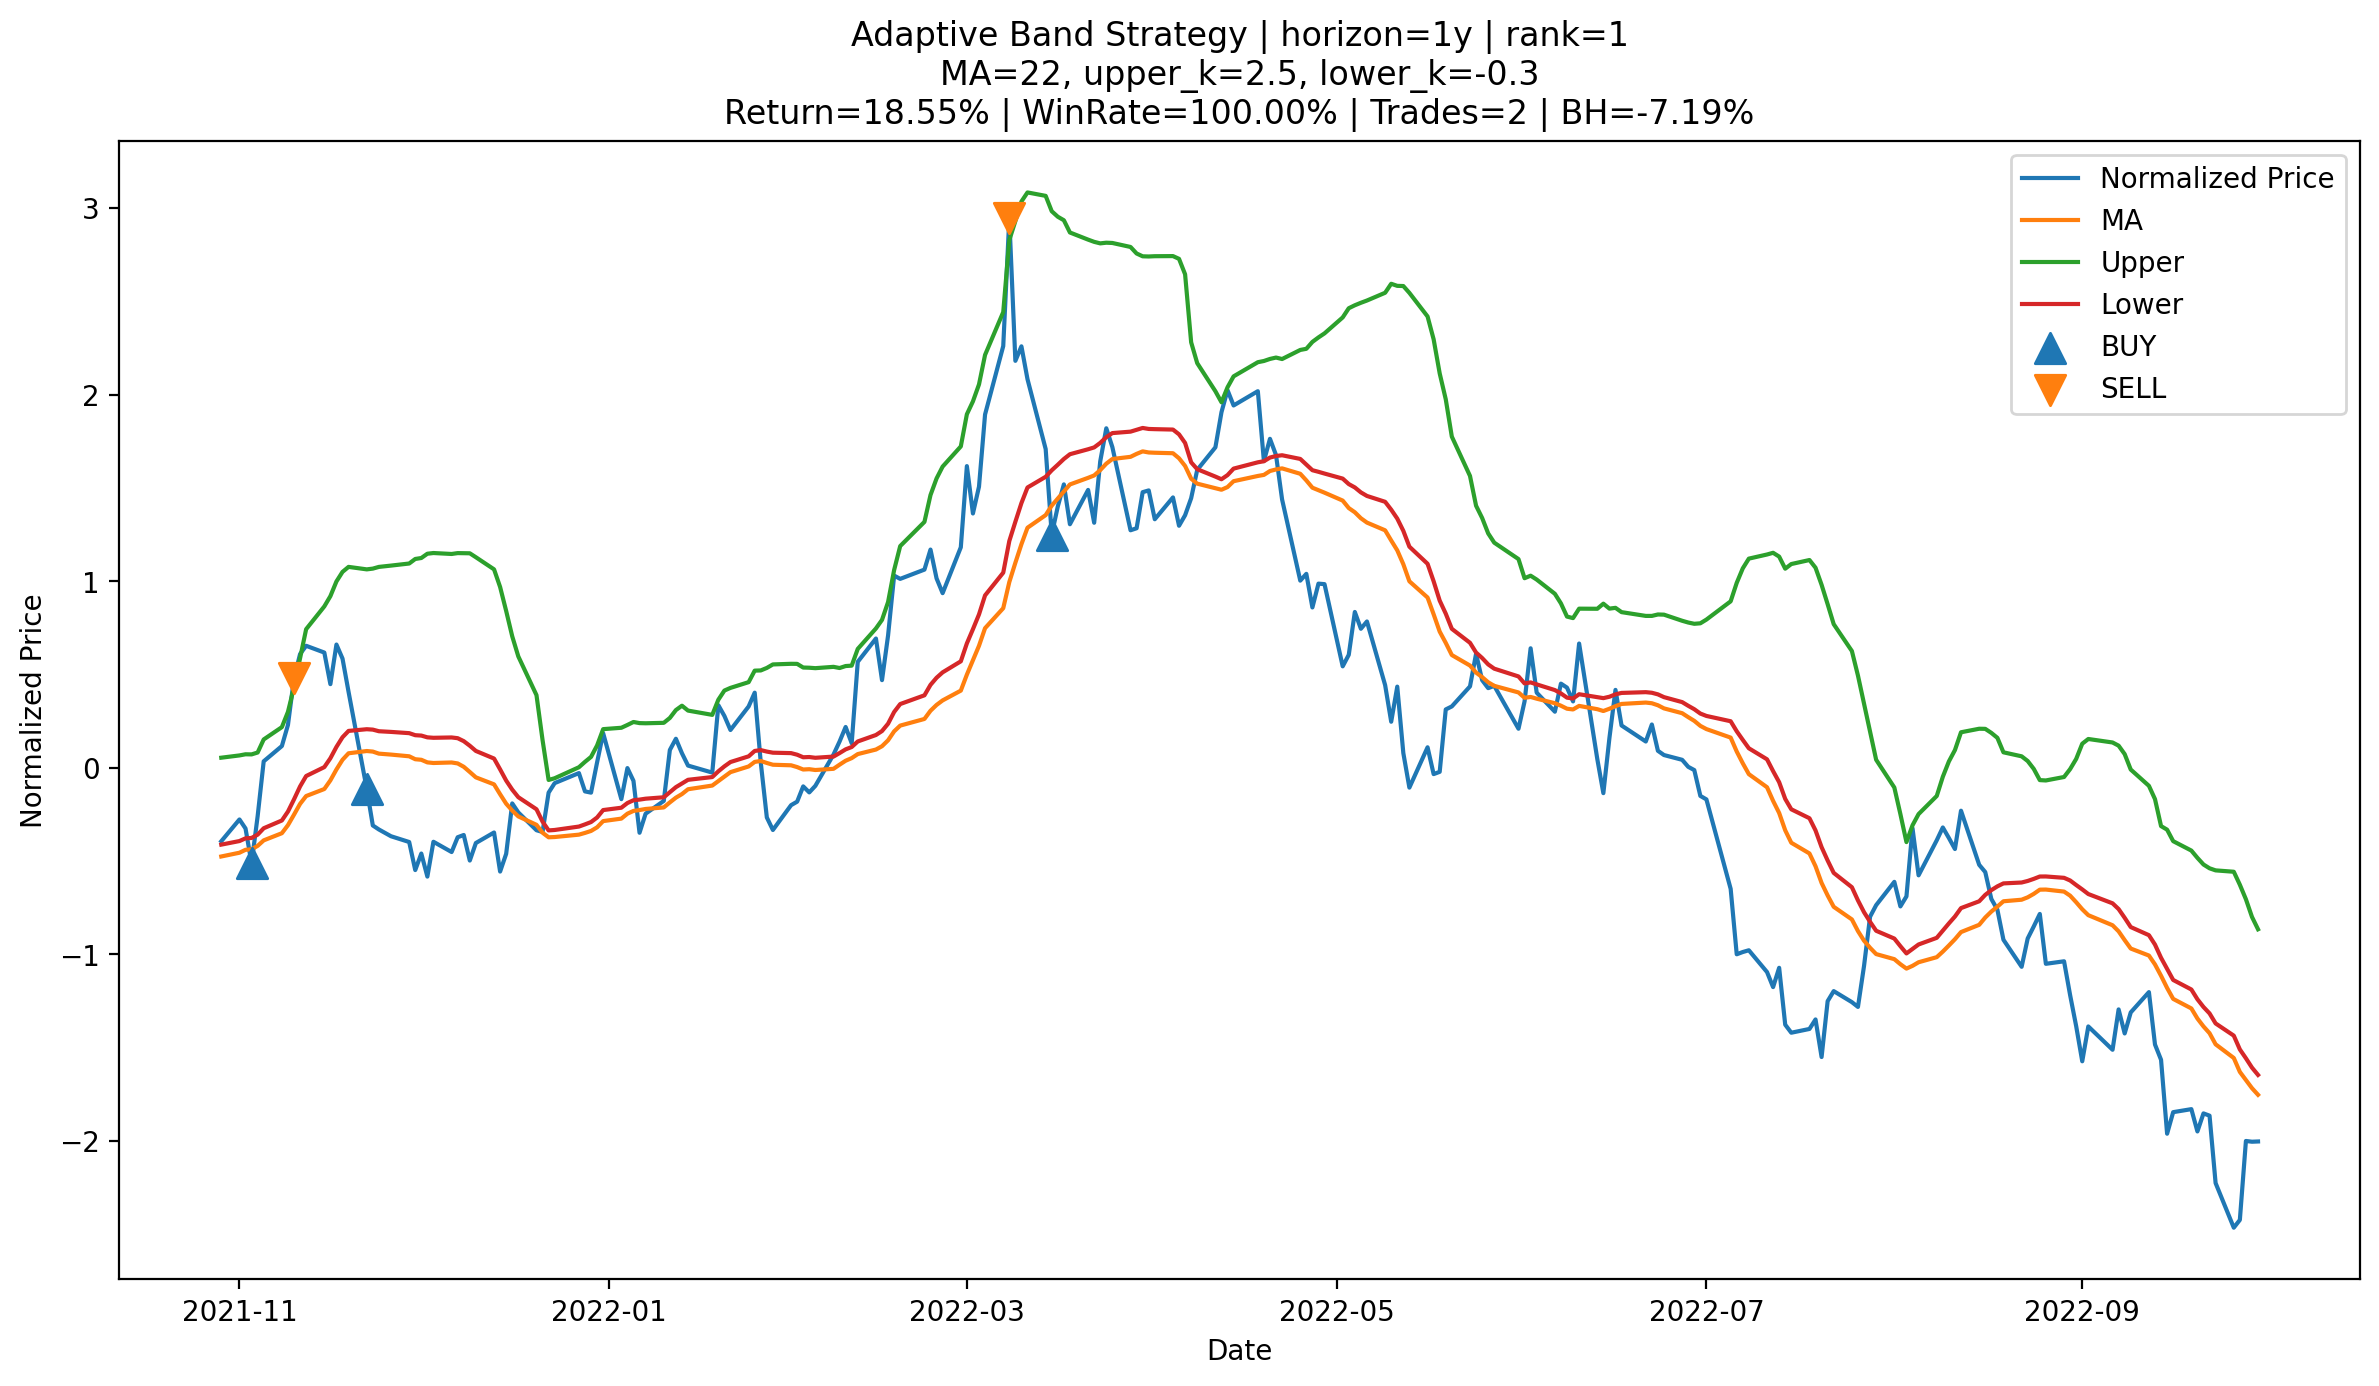
\includegraphics[width=\textwidth]{../../figures/adaptive_band_strategy/1y/1y_rank01_ma22_uk2.5_lk-0.3.png}
    \end{column}
  \end{columns}
\end{frame}

% ── Slide 6: Strategy 2 ──────────────────────────────────────────────────────
\begin{frame}{Strategy 2: Moving-Average Crossover}
  \begin{columns}[T]
    \begin{column}{0.40\textwidth}
      \small
      \textbf{Signal type: continuous}
      \vspace{0.5em}
      \begin{itemize}
        \item Short-window MA compared against long-window MA
        \item Positive spread: uptrend; negative spread: downtrend
        \item Score captures direction and magnitude of the gap
        \item Buy: short MA crosses above long MA
        \item Sell: short MA crosses below long MA
      \end{itemize}
    \end{column}
    \begin{column}{0.57\textwidth}
      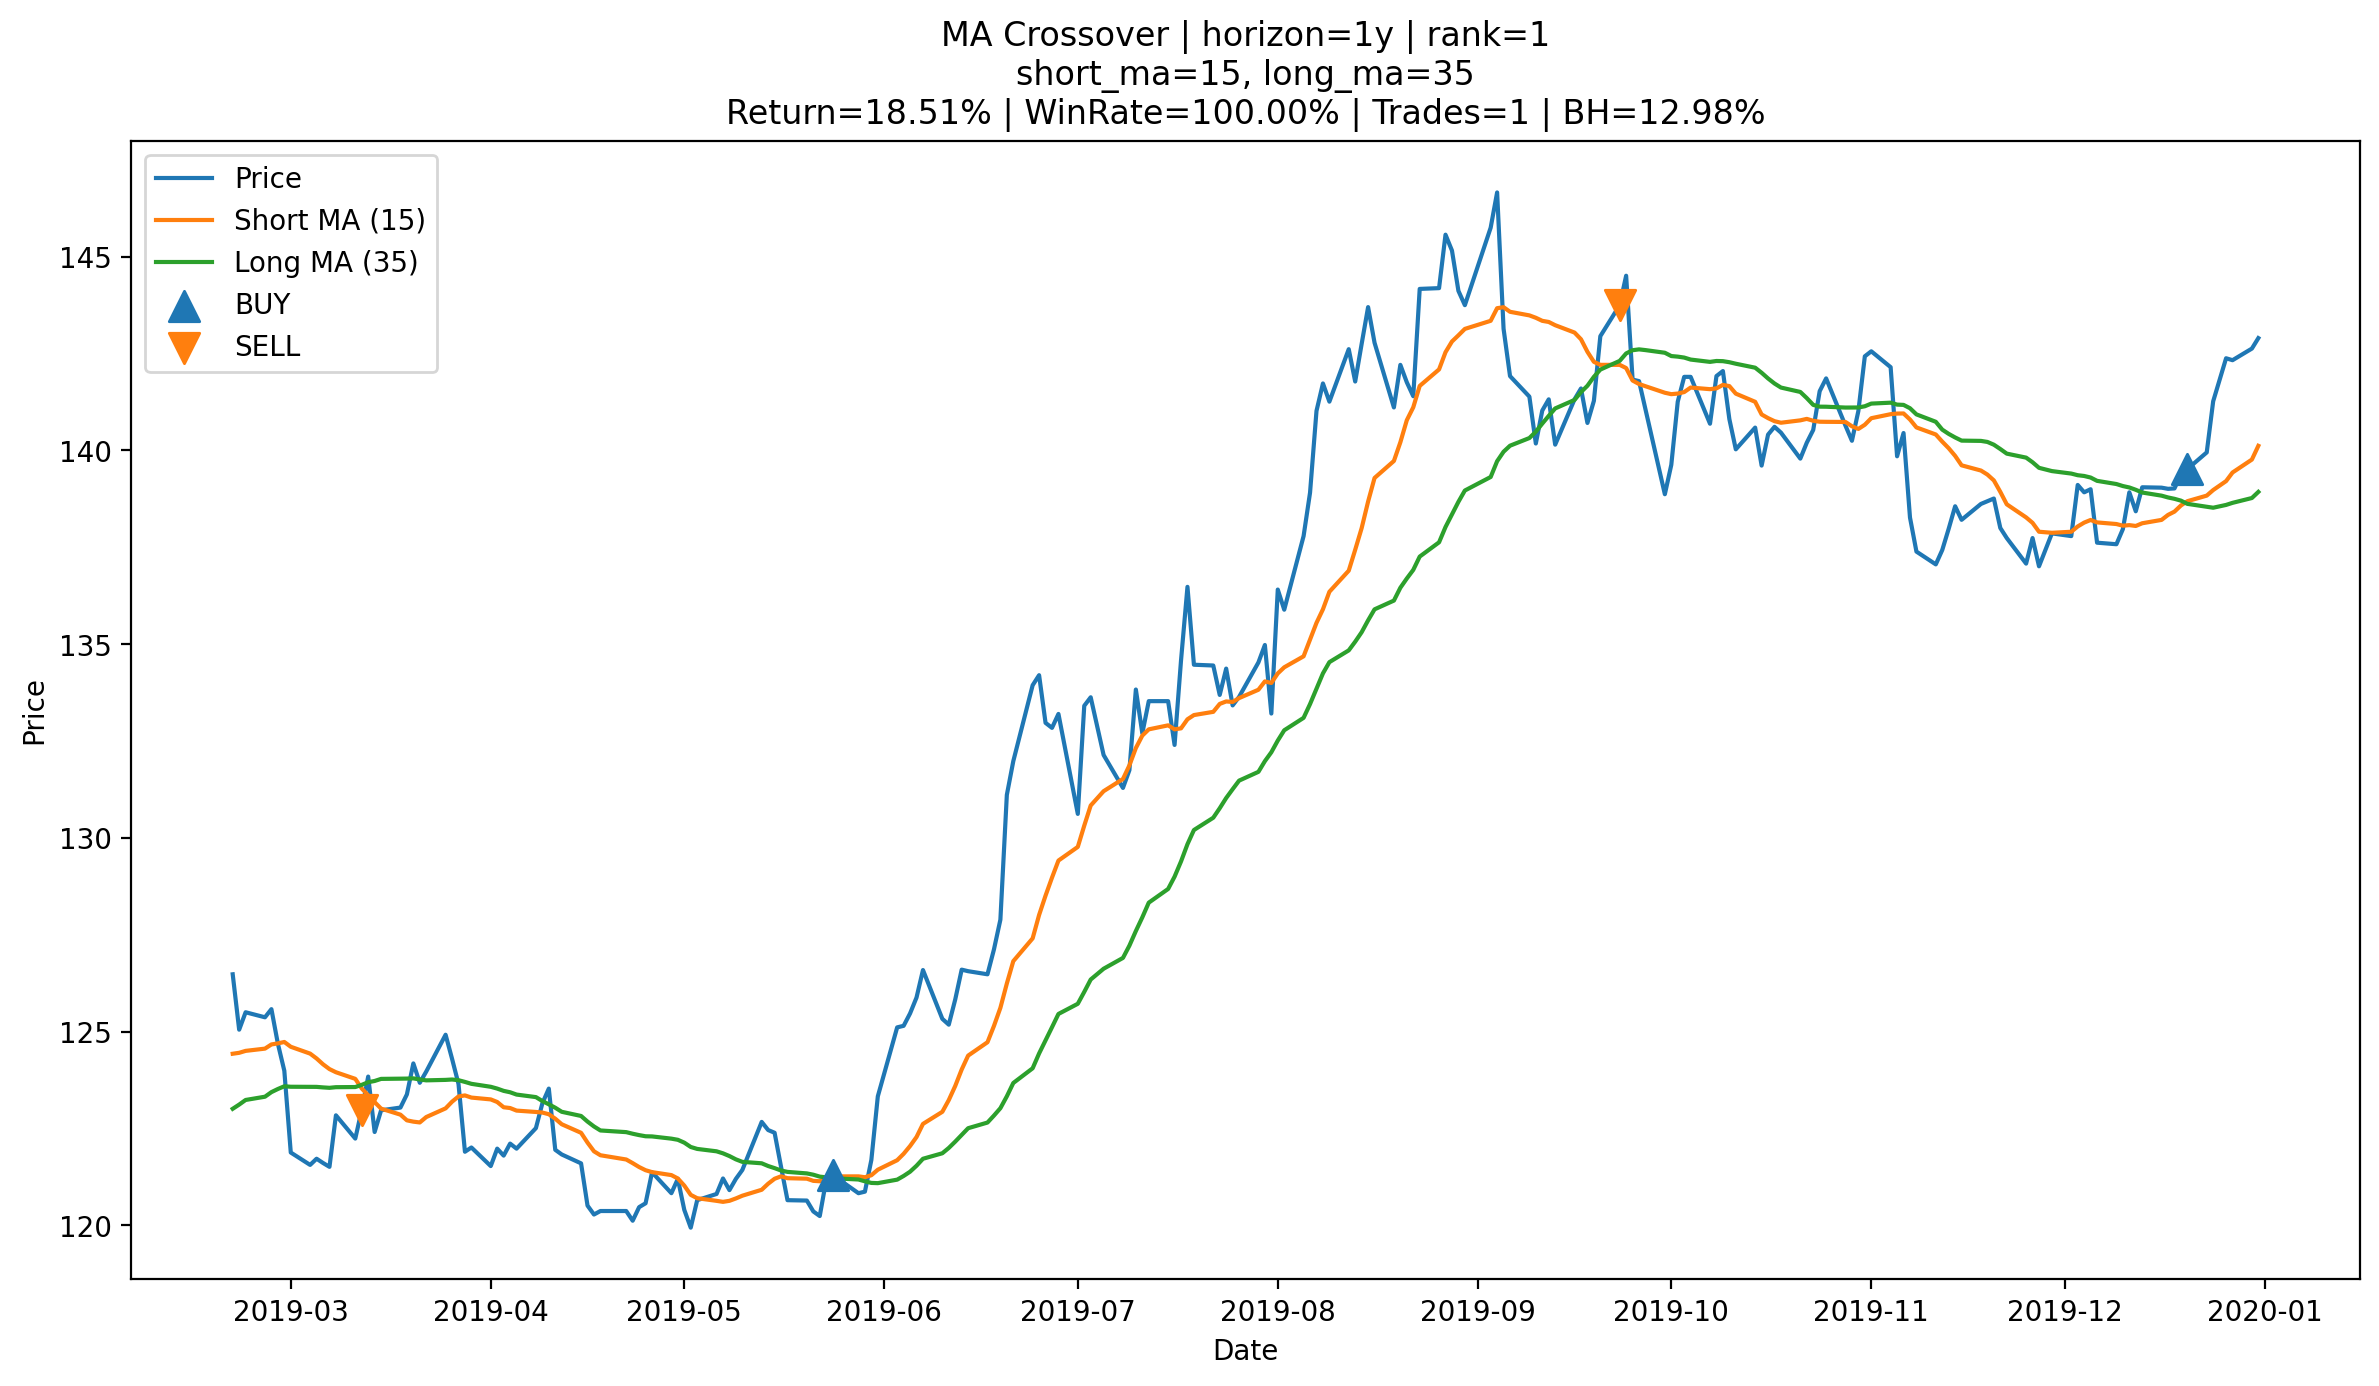
\includegraphics[width=\textwidth]{../../figures/ma_crossover/1y/1y_rank01_sma15_lma35.png}
    \end{column}
  \end{columns}
\end{frame}

% ── Slide 7: Strategy 3 ──────────────────────────────────────────────────────
\begin{frame}{Strategy 3: Adaptive Volatility Band}
  \begin{columns}[T]
    \begin{column}{0.40\textwidth}
      \small
      \textbf{Signal type: continuous}
      \vspace{0.5em}
      \begin{itemize}
        \item Volatility proxy from high-low-close range
        \item Bands placed relative to rolling volatility level
        \item Score reflects current volatility regime position
        \item High-vol breakouts and low-vol compressions produce distinct signals
        \item Complementary to price-band strategies
      \end{itemize}
    \end{column}
    \begin{column}{0.57\textwidth}
      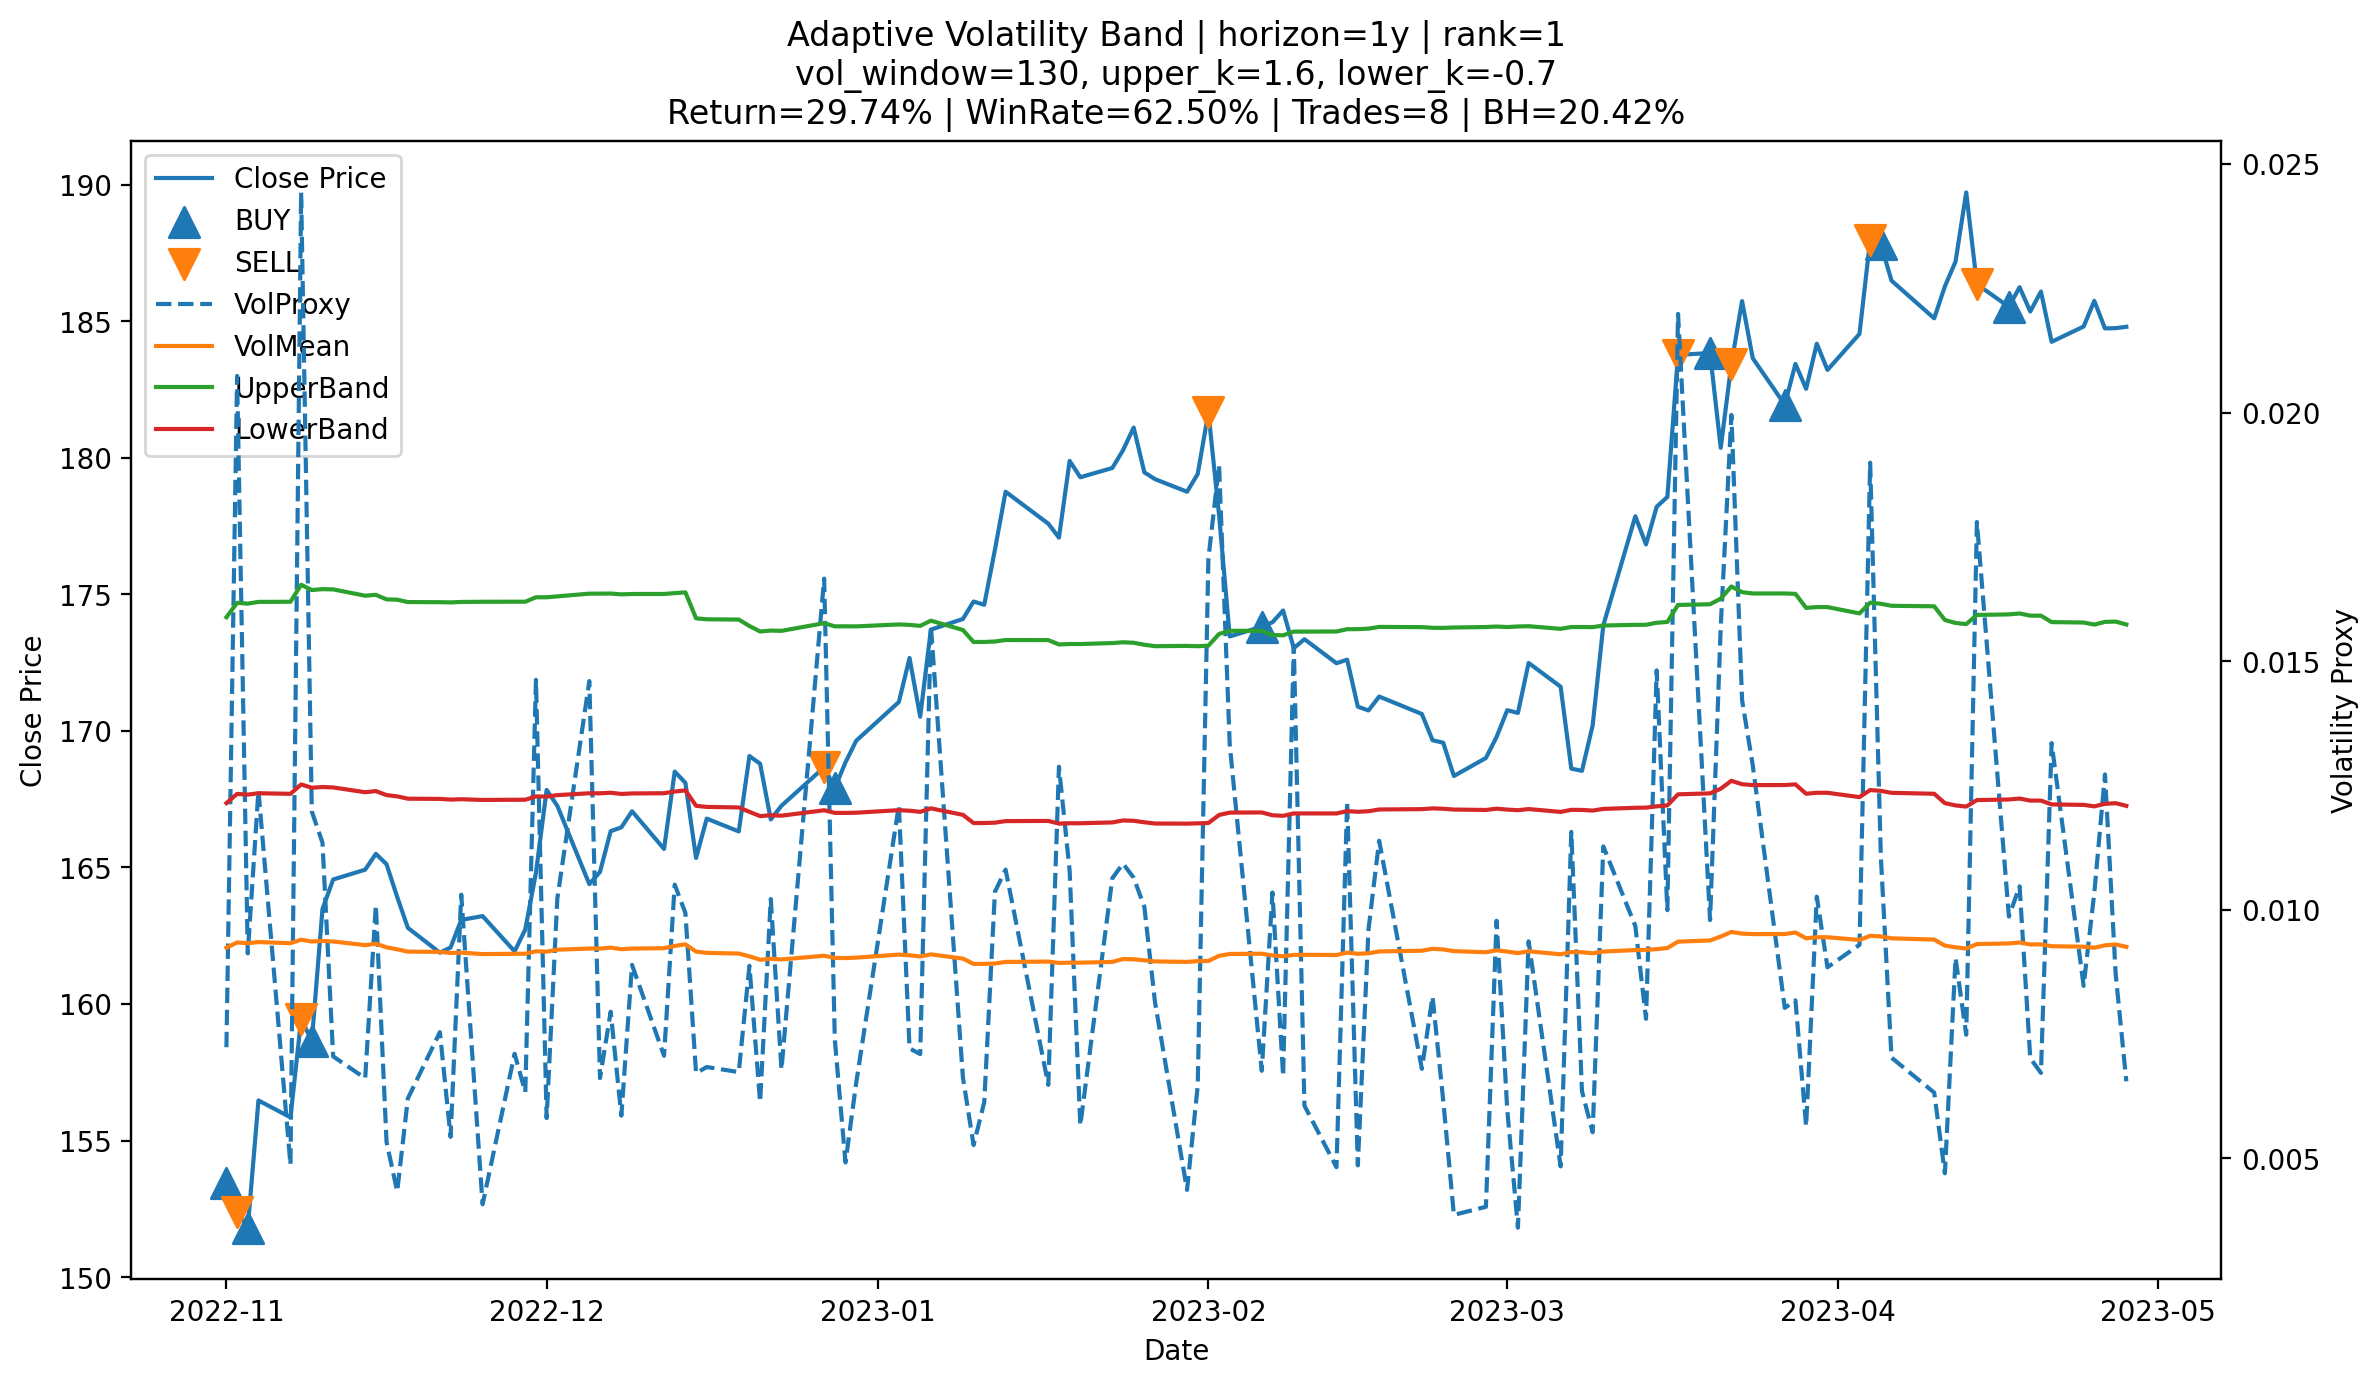
\includegraphics[width=\textwidth]{../../figures/adaptive_volatility_band_strategy/1y/1y_rank01_vw130_uk1.6_lk-0.7.png}
    \end{column}
  \end{columns}
\end{frame}

% ── Slide 8: Strategy 4 ──────────────────────────────────────────────────────
\begin{frame}{Strategy 4: Fear-Greed Candle-Volume}
  \begin{columns}[T]
    \begin{column}{0.40\textwidth}
      \small
      \textbf{Signal type: event-style}
      \vspace{0.5em}
      \begin{itemize}
        \item Fires only when candle body size \textbf{and} volume spike simultaneously
        \item Captures extreme sentiment: large directional move confirmed by activity
        \item Rare by design; most days produce no signal
        \item Qualitatively different from the three continuous strategies
        \item Adds a sparse basis vector to matrix \(A\)
      \end{itemize}
    \end{column}
    \begin{column}{0.57\textwidth}
      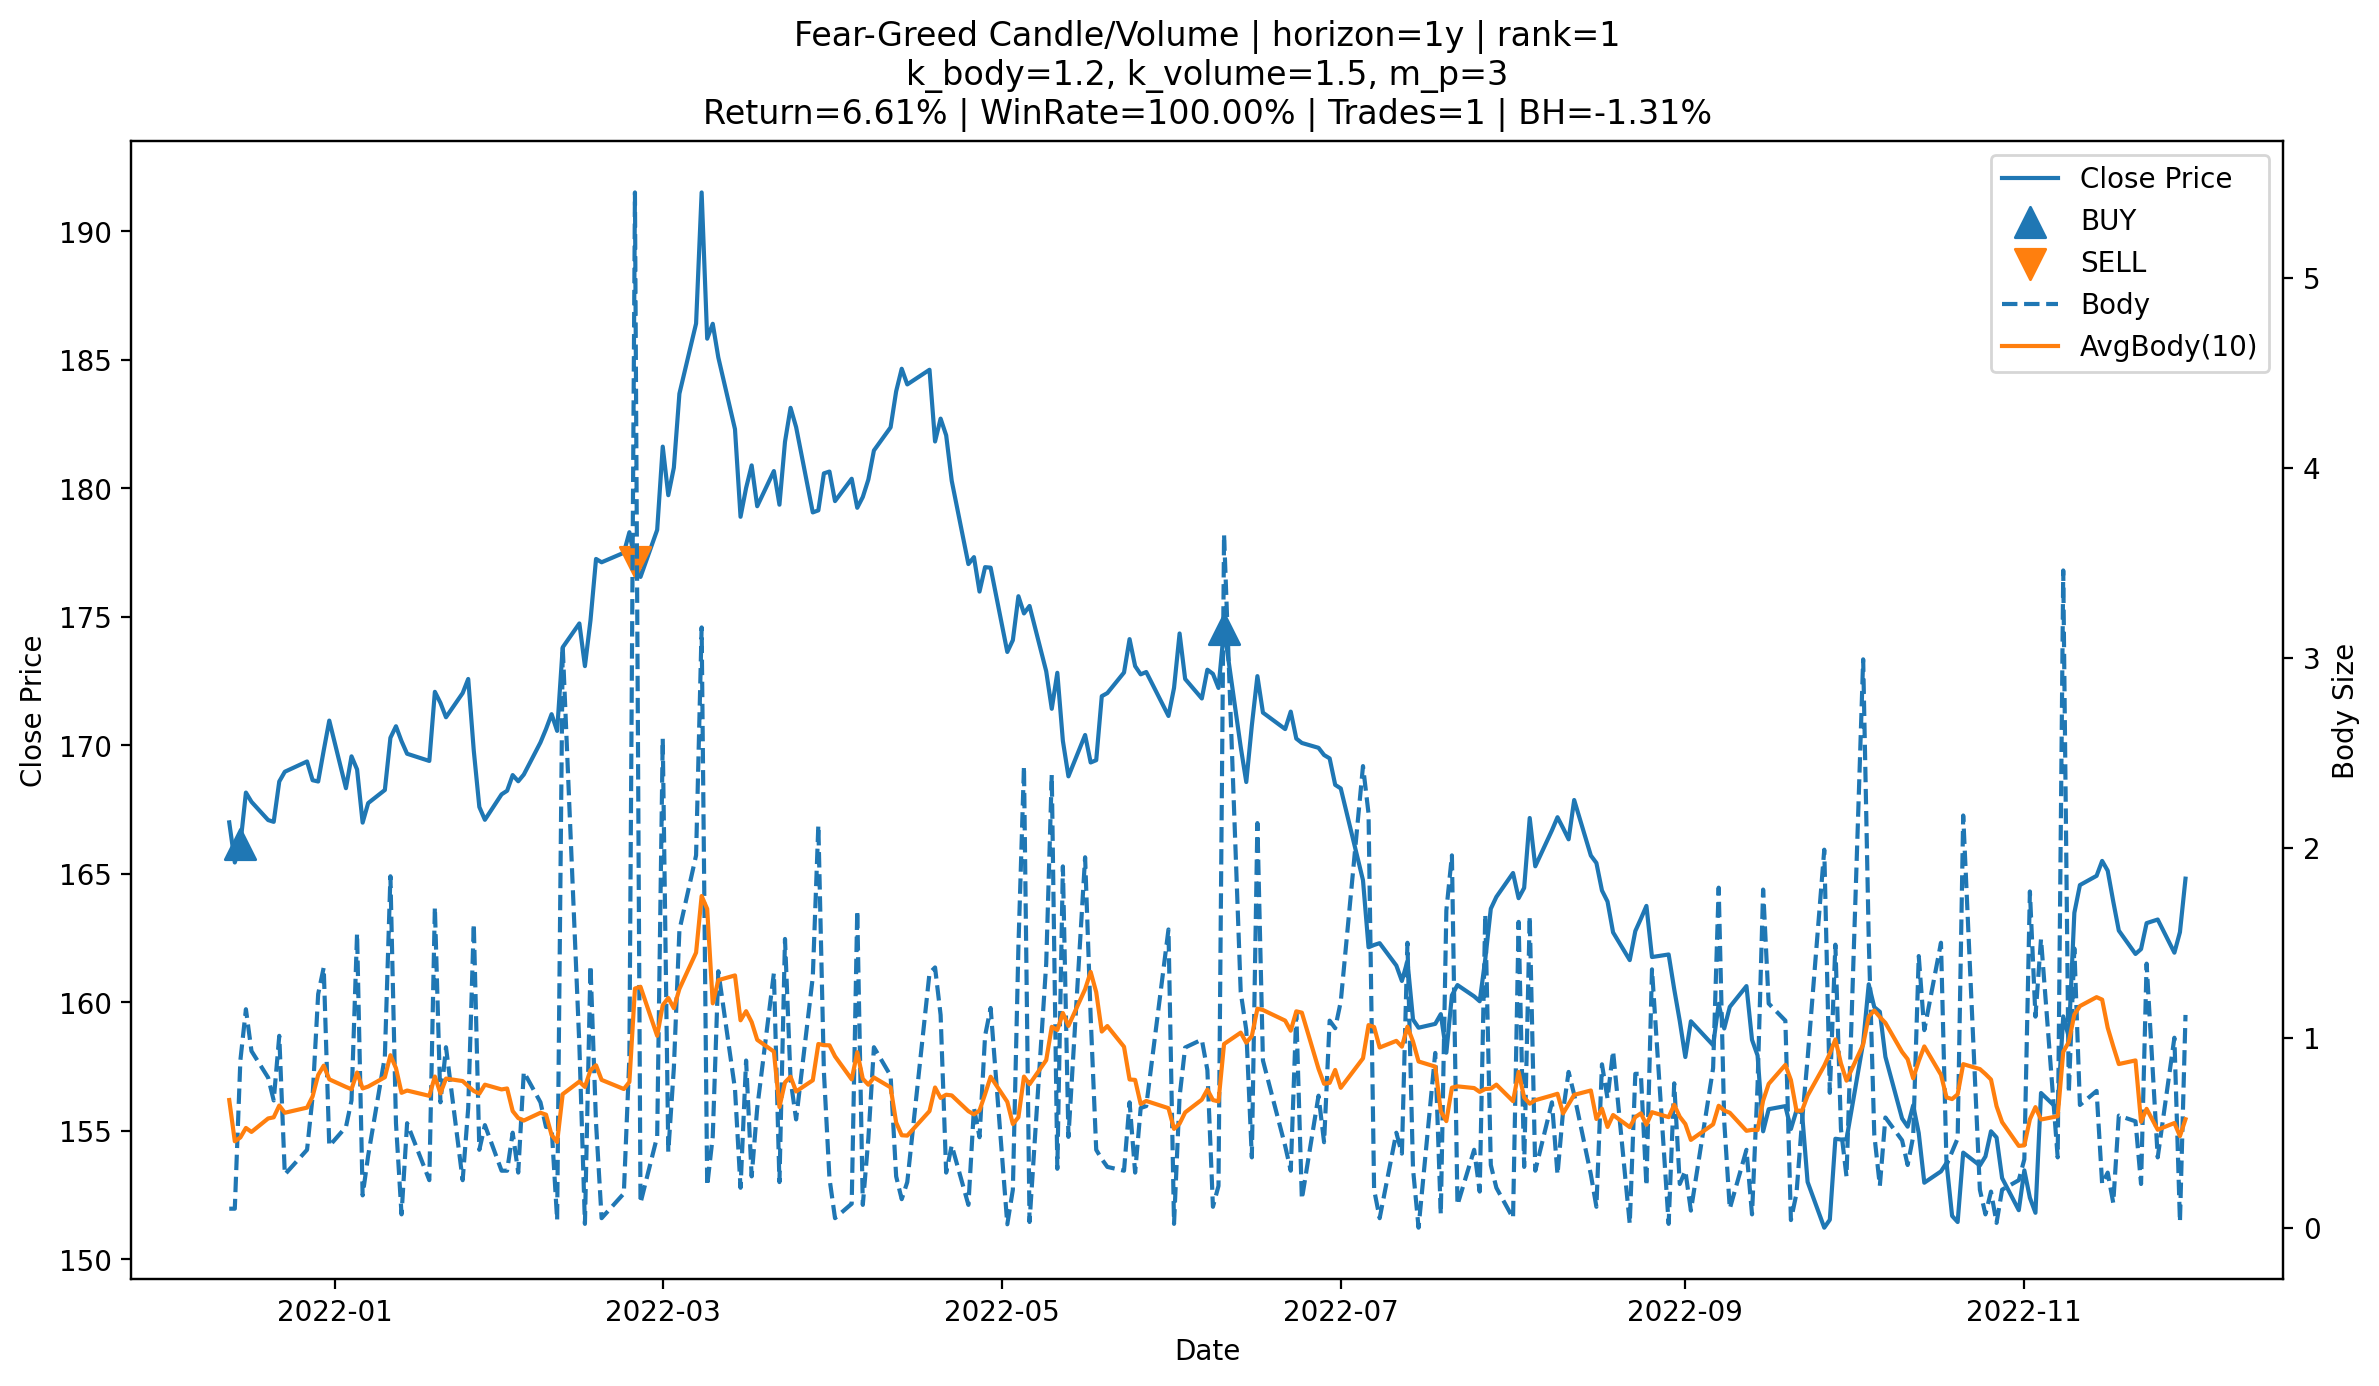
\includegraphics[width=\textwidth]{../../figures/fear_greed_candle_volume_strategy/1y/1y_rank01_kb1.2_kv1.5_mp3.png}
    \end{column}
  \end{columns}
\end{frame}

% ── Slide 9: Parameters as Functions ────────────────────────────────────────
\begin{frame}{Turning Parameters into Signals}
  Each strategy family has its own parameters. After optimization, the best
  parameters define a concrete signal function for that anchor.

  \vspace{0.5em}
  \textbf{Example: anchor date 2021-12-31}

  \vspace{0.4em}
  \textbf{Strategy 1 — Adaptive Band} \hfill (MA=65, upper\_k=0.0, lower\_k=0.6)
  \[
    s_{\text{band}}(t) = \frac{P_t - \text{MA}_{65}(t)}{\sigma_{65}(t)},
    \quad \text{buy signal when } s_{\text{band}}(t) < 0.6
  \]

  \vspace{0.3em}
  \textbf{Strategy 2 — MA Crossover} \hfill (short=60, long=65)
  \[
    s_{\text{ma}}(t) = \text{MA}_{60}(t) - \text{MA}_{65}(t),
    \quad \text{buy signal when } s_{\text{ma}}(t) > 0
  \]

  \vspace{0.5em}
  \begin{itemize}
    \item Parameters are re-optimized at every anchor date (monthly)
    \item Each anchor produces a different function adapted to recent market behavior
    \item The score value on any day becomes one entry in matrix \(A\)
  \end{itemize}
\end{frame}

% ── Stage A — Single Strategy Results ───────────────────────────────────────
\begin{frame}{Stage A: What Happens with One Strategy at a Time?}
  \small
  Hold 130 days $\cdot$ 1-month parameter update $\cdot$ rank-1 parameters per anchor

  \vspace{0.5em}
  \begin{tabular}{lrrrrr}
    \toprule
    Year & B\&H & Adap.Band & MA Cross & Adap.Vol & Fear-Greed \\
    \midrule
    2020 & +23.9\% & +4.4\% & +5.2\% & +5.8\% & $\approx$0\% \\
    2021 & $-$6.2\%  & +0.3\% & $-$0.2\% & +0.9\% & $\approx$0\% \\
    2022 & +0.8\%  & $-$0.9\% & $-$3.0\% & $-$2.1\% & $\approx$0\% \\
    2023 & +11.8\% & +1.5\% & +0.9\% & +2.1\% & $\approx$0\% \\
    2024 & +27.0\% & +5.9\% & +6.3\% & +10.6\% & $\approx$0\% \\
    \bottomrule
  \end{tabular}

  \vspace{0.6em}
  \begin{itemize}
    \item Each strategy alone captures only a \textbf{fraction} of the market move
    \item Exposure is low (21--46\%): the strategy sits out most days
    \item Fear-Greed: after removing look-ahead bug, GLD rarely triggers the threshold ($\approx$0\% exposure)
  \end{itemize}
\end{frame}

% ── Slide 10: Matrix A and the Combination Problem ───────────────────────────
\begin{frame}{Stage B: Combining Strategies — Matrix A}
  \textbf{Idea:} instead of picking one strategy, weight all four.

  \vspace{0.6em}
  Define the design matrix \(A\) where each column is one strategy score:
  \[
    A \;=\;
    \begin{pmatrix}
      s_1(t_1) & s_2(t_1) & s_3(t_1) & s_4(t_1) \\
      s_1(t_2) & s_2(t_2) & s_3(t_2) & s_4(t_2) \\
      \vdots   & \vdots   & \vdots   & \vdots   \\
      s_1(t_n) & s_2(t_n) & s_3(t_n) & s_4(t_n)
    \end{pmatrix}
  \]

  \vspace{0.4em}
  Find weights \(\mathbf{x} \geq 0\) (long-only) that maximize realized return \(y\):
  \[
    \max_{\mathbf{x} \geq 0,\; \mathbf{1}^\top \mathbf{x} = 1}
    \quad y(\mathbf{x}) \;=\; \text{portfolio return using combined signal } A\mathbf{x}
  \]

  \vspace{0.4em}
  This is \textbf{Objective 1}: a constrained optimization over the strategy space.\\
  Parameters are re-optimized at each anchor date (rolling walk-forward).
\end{frame}

% ── Stage B Weights Example ──────────────────────────────────────────────────
\begin{frame}{Stage B: What Did the Optimizer Actually Find?}
  \textbf{Anchor: 2021-12-31} — selection period return vs.\ buy-and-hold: \textbf{+10.2\% vs $-$6.2\%}

  \vspace{0.5em}
  Long-only weight optimization over the 4 strategy signals:

  \[
    \hat{s}(t) \;=\; \underbrace{0.45}_{\text{Adaptive Band}} \cdot s_{\text{band}}(t)
              \;+\; \underbrace{0.00}_{\text{MA Cross}} \cdot s_{\text{ma}}(t)
              \;+\; \underbrace{0.55}_{\text{Adap.Vol}} \cdot s_{\text{vol}}(t)
              \;+\; \underbrace{0.00}_{\text{Fear-Greed}} \cdot s_{\text{fg}}(t)
  \]

  \vspace{0.5em}
  \begin{itemize}
    \item Two strategies dominate: Adaptive Band (45\%) and Adaptive Vol (55\%)
    \item MA Crossover and Fear-Greed received zero weight — optimizer excluded them
    \item This mirrors Lasso-style selection: only the most informative signals survive
    \item Standalone returns in selection period: Band=+10.0\%, Vol=+10.1\%, MA=$-$5.6\%
  \end{itemize}

  \vspace{0.3em}
  \small The combined signal \(\hat{s}(t)\) then drives portfolio exposure via the tranche system.
\end{frame}

% ── Stage B Results ───────────────────────────────────────────────────────────
\begin{frame}{Stage B: Ensemble Results}
  \small
  Hold 130 days $\cdot$ 1-month update $\cdot$ long-only weight re-optimization per anchor

  \vspace{0.5em}
  \begin{tabular}{lrrrr}
    \toprule
    Year & B\&H & Stage A (best single) & Stage B (ensemble) & Improvement \\
    \midrule
    2020 & +23.9\% & +4.4\% & +6.4\% & $\uparrow$ \\
    2021 & $-$6.2\%  & +0.3\% & +0.3\% & $\sim$ \\
    2022 & +0.8\%  & $-$0.9\% & $-$2.3\% & $\downarrow$ \\
    2023 & +11.8\% & +1.6\% & +2.0\% & $\uparrow$ \\
    2024 & +27.0\% & +5.9\% & +8.0\% & $\uparrow$ \\
    \bottomrule
  \end{tabular}

  \vspace{0.6em}
  \begin{itemize}
    \item Ensemble beats single strategy in 3/5 years, but margin is small
    \item Exposure stays low (23--42\%): combined signal is still weak
    \item 2022: ensemble \emph{worse} than best single ($-$2.3\% vs $-$0.9\%) --- diversification hurts in whipsaw markets
    \item \textbf{The weights are fixed after optimization --- they cannot adapt to what the market is doing now}
  \end{itemize}
\end{frame}

% ── Slide 12: Motivation for Stage C ────────────────────────────────────────
\begin{frame}{What Stage B Cannot Do}
  Stage B finds the best \emph{historical} weight vector \(\mathbf{x}\).

  \vspace{0.6em}
  But the market changes. The optimal combination today may differ from last month.

  \vspace{0.6em}
  \textbf{The missing step:}
  \[
    \text{learn how to combine signals to predict } \textbf{future} \text{ return}
  \]

  \vspace{0.6em}
  \begin{tabular}{lll}
    \toprule
    & Stage B & Stage C \\
    \midrule
    Question    & best historical weights? & what predicts future return? \\
    Method      & constrained optimization & supervised learning \\
    Signal use  & combine realized returns & use current scores as features \\
    Adaptation  & fixed per anchor         & model selected per anchor \\
    \bottomrule
  \end{tabular}
\end{frame}

% ── Slide 13: Stage C — Expanded Space ──────────────────────────────────────
\begin{frame}{Stage C: Expanding the Strategy Space}
  \textbf{Objective 2}: treat strategy scores as \emph{features} for a supervised model.

  \vspace{0.5em}
  Expand from 4 to \textbf{40 basis columns}:
  \[
    A \in \mathbb{R}^{n \times 40}
    \quad \text{(top 10 parameter sets per strategy family)}
  \]

  \vspace{0.4em}
  This mirrors the class model-selection exercise:
  \[
    \text{many basis functions} \;\longrightarrow\; \text{select useful structure}
  \]

  \vspace{0.4em}
  Four linear models compared:
  \[
    \text{OLS} \quad \text{Ridge} \quad \text{Lasso} \quad \text{Elastic Net}
  \]

  \vspace{0.4em}
  Model selection criterion: \textbf{time-series cross-validated MSE} (no look-ahead).
\end{frame}

% ── Slide 14: Stage C — Forward Validation ───────────────────────────────────
\begin{frame}{Stage C: Forward Validation Design}
  \begin{columns}[T]
    \begin{column}{0.50\textwidth}
      \textbf{Anchor-date setup}
      \vspace{0.5em}
      \begin{itemize}
        \item Monthly anchor dates: 2020--2024
        \item \textbf{Selection period}: 1 year before anchor
        \begin{itemize}
          \item fit model, pick best model by CV-MSE
        \end{itemize}
        \item \textbf{Evaluation period}: after anchor
        \begin{itemize}
          \item apply frozen model to unseen data
        \end{itemize}
        \item Model re-fitted at each new anchor
      \end{itemize}
    \end{column}
    \begin{column}{0.47\textwidth}
      \vspace{1em}
      \[
        \underbrace{\longleftarrow\text{1 year}\longrightarrow}_{\text{selection}}
        \Big|_{\text{anchor}}
        \underbrace{\longrightarrow}_{\text{evaluation}}
      \]
      \vspace{1em}
      \small
      The model never sees future data during fitting.\\[0.5em]
      This separates model discovery from forward validation.
    \end{column}
  \end{columns}
\end{frame}

% ── Slide 15: Stage C — Prediction to Portfolio Weight ───────────────────────
\begin{frame}{Stage C: From Prediction to Portfolio Weight}
  The model outputs a predicted future cumulative return \(\hat{y}_t\).

  \vspace{0.6em}
  Convert to a long-only portfolio weight:
  \[
    w_t \;=\; \operatorname{clip}\!\left(\frac{\hat{y}_t}{s},\; 0,\; 1\right)
  \]
  where \(s\) is a quantile-based scale factor from the selection period.

  \vspace{0.6em}
  Execute via rolling tranches:
  \begin{itemize}
    \item Each day: compute signal, open one tranche at weight \(w_t\)
    \item Hold for fixed horizon (45 or 130 days), then close
    \item Gross exposure = average of all open tranches
  \end{itemize}

  \vspace{0.5em}
  \textbf{Key property}: when the model is confident (\(\hat{y}_t\) large), exposure rises.\\
  When uncertain (\(\hat{y}_t \approx 0\)), exposure falls naturally.
\end{frame}

% ── Slide 16: Three-Stage Comparison — KEY SLIDE ────────────────────────────
\begin{frame}{Three-Stage Comparison: A vs B vs C}
  \small
  Hold 130 days $\cdot$ 1-month update $\cdot$ \textbf{Ret / Exposure / Efficiency (Ret $\div$ Exp)}

  \vspace{0.4em}
  \begin{tabular}{lrp{2.8cm}p{2.8cm}p{3.0cm}}
    \toprule
    Year & B\&H & A: Single Signal & B: Ensemble & C: ML-Guided \\
    \midrule
    2020 & +23.9\% & +4.4\% / 27\% / +16\%  & +6.4\% / 32\% / +20\% & \textbf{+10.9\%} / 57\% / \textbf{+19\%} \\
    2021 & $-$6.2\%  & +0.3\% / 25\% / +1\%  & +0.3\% / 25\% / +1\%  & \textbf{+0.8\%} / 29\% / \textbf{+3\%} \\
    2022 & +0.8\%  & $-$0.9\% / 46\% / $-$2\% & $-$2.3\% / 42\% / $-$5\% & \textbf{$-$0.2\%} / 31\% / \textbf{$-$1\%} \\
    2023 & +11.8\% & +1.6\% / 25\% / +6\%  & +2.0\% / 23\% / +9\%  & \textbf{+4.0\%} / 32\% / \textbf{+12\%} \\
    2024 & +27.0\% & +5.9\% / 21\% / +29\% & +8.0\% / 29\% / +27\% & \textbf{+16.4\%} / 65\% / \textbf{+25\%} \\
    \bottomrule
  \end{tabular}

  \vspace{0.5em}
  \begin{itemize}
    \item C outperforms A and B in \textbf{every year} on both return and efficiency
    \item 2024: A(+5.9\%) $\to$ B(+8.0\%) $\to$ \textbf{C(+16.4\%)} — clear step-up at each stage
    \item \textbf{Core insight}: ML-Guided learns \emph{when} and \emph{how much} to bet, not just which strategy
  \end{itemize}
\end{frame}

% ── Stage C Model Example ────────────────────────────────────────────────────
\begin{frame}{Stage C: What Does the Chosen Model Look Like?}
  \textbf{Anchor: 2021-11-30} — OLS selected, horizon=130 days, corr=0.995

  \vspace{0.3em}
  From 40 basis columns, the top contributing features (by absolute coefficient):

  \vspace{0.3em}
  \small
  \begin{tabular}{llr}
    \toprule
    Feature & Strategy family & Coefficient \\
    \midrule
    \texttt{ma\_crossover\_rank07}       & MA Crossover   & $-0.212$ \\
    \texttt{adaptive\_band\_rank05}      & Adaptive Band  & $+0.099$ \\
    \texttt{adaptive\_band\_rank06}      & Adaptive Band  & $+0.097$ \\
    \texttt{adaptive\_band\_rank03}      & Adaptive Band  & $-0.075$ \\
    \texttt{adaptive\_band\_rank04}      & Adaptive Band  & $-0.073$ \\
    \texttt{ma\_crossover\_rank10}       & MA Crossover   & $+0.071$ \\
    $\vdots$ & $\vdots$ & $\vdots$ \\
    \bottomrule
  \end{tabular}

  \normalsize
  \vspace{0.5em}
  \begin{itemize}
    \item 28 out of 40 features are nonzero — OLS uses the full correlated space
    \item The model mixes \emph{ranks within a strategy}, not just strategies
    \item Prediction: \(\hat{y}_t = \beta_0 + \sum_{j=1}^{40} \beta_j \cdot A_{tj}\)
    \item \(\hat{y}_t\) becomes the portfolio weight \(w_t = \operatorname{clip}(\hat{y}_t / s,\; 0,\; 1)\)
  \end{itemize}
\end{frame}

% ── Update Frequency ──────────────────────────────────────────────────────────
\begin{frame}{How Often Should the Model Update?}
  \small
  \begin{tabular}{lrrrrr}
    \toprule
    Year & B\&H & 1M & 2M & 3M & 6M \\
    \midrule
    2020 & +23.9\% & +10.9\% / 57\% & +10.2\% / 57\% & +9.6\% / 51\% & +9.7\% / 50\% \\
    2021 & $-$6.2\%  & +0.8\% / 29\% & +0.3\% / 35\% & +0.6\% / 28\% & $-$0.7\% / 49\% \\
    2022 & +0.8\%  & $-$0.2\% / 31\% & +0.9\% / 35\% & $-$0.8\% / 33\% & $-$1.7\% / 44\% \\
    2023 & +11.8\% & +4.0\% / 32\% & +4.1\% / 23\% & +3.8\% / 40\% & +3.4\% / 15\% \\
    2024 & +27.0\% & +16.4\% / 65\% & +13.9\% / 60\% & +11.1\% / 53\% & +5.5\% / 36\% \\
    \bottomrule
  \end{tabular}

  \vspace{0.6em}
  \begin{itemize}
    \item \textbf{1M consistently best}: fastest adaptation captures regime shifts
    \item Longer intervals miss the 2024 bull run (6M: +5.5\% vs 1M: +16.4\%)
    \item Trade-off: more frequent updates require more compute but pay off
  \end{itemize}
\end{frame}

% ── Slide 18: What's Next? ───────────────────────────────────────────────────
\begin{frame}{What's Next? — Three Natural Extensions}

  \textbf{1. Nonlinear Model Selection via SINDy}
  \begin{itemize}
    \item Current: linear basis $A\beta \approx y$ with OLS / Ridge / Lasso
    \item SINDy expands the library with nonlinear terms:
    \[
      \Theta(A) = \bigl[\,s_i,\; s_i^2,\; s_i s_j,\; \sin(s_i),\; \dots\,\bigr]
    \]
    \item Sparse regression then selects only the terms that matter
    \item If linear combinations already work, nonlinear interactions may do better
  \end{itemize}

  \vspace{0.4em}
  \textbf{2. Hierarchical Strategy Structure — Deep Learning}
  \begin{itemize}
    \item Current: 4 strategies work in \emph{parallel} (flat design matrix)
    \item What if strategies form \emph{layers}? \\
          Layer 1: direction signals \(\;\longrightarrow\;\) Layer 2: timing signals
    \item Each layer applies a nonlinear transform — this is a neural network
    \item Analogy: listen to one analyst for the trend, then another for the entry
  \end{itemize}

  \vspace{0.4em}
  \textbf{3. Multi-Asset Expansion}
  \begin{itemize}
    \item Same framework applied across GLD, oil, copper, equities
    \item Cross-asset signals become additional columns of $A$
    \item Captures regime correlation across markets
  \end{itemize}

\end{frame}

% ── Slide 19: Conclusion ─────────────────────────────────────────────────────
\begin{frame}{Conclusion}
  \begin{block}{Main Finding}
    Treating trading strategy outputs as basis functions creates a valid,
    predictive strategy space. ML model selection over that space substantially
    outperforms both single-strategy and ensemble approaches.
  \end{block}

  \vspace{0.6em}
  \begin{tabular}{ll}
    \toprule
    Stage & Key Takeaway \\
    \midrule
    A: Single Signal  & Exposure 21--46\%; captures small fraction of market move \\
    B: Ensemble       & Diversification alone does not improve prediction \\
    C: ML-Guided      & Learns \emph{when} to be exposed; 2024: $\times$2.0 vs B, $\times$2.8 vs A \\
    \bottomrule
  \end{tabular}

  \vspace{0.6em}
  \textbf{Next steps:}
  \begin{itemize}
    \item Multi-asset expansion (oil, copper, equities)
    \item Regime-aware exposure control layer
    \item Live deployment via Raspberry Pi + Alpaca paper trading
  \end{itemize}
\end{frame}

\end{document}
